%% abtex2-modelo-projeto-pesquisa.tex, v-1.9.7 laurocesar
%% Copyright 2012-2018 by abnTeX2 group at http://www.abntex.net.br/
%%
%% This work may be distributed and/or modified under the
%% conditions of the LaTeX Project Public License, either version 1.3
%% of this license or (at your option) any later version.
%% The latest version of this license is in
%%   http://www.latex-project.org/lppl.txt
%% and version 1.3 or later is part of all distributions of LaTeX
%% version 2005/12/01 or later.
%%
%% This work has the LPPL maintenance status `maintained'.
%%
%% The Current Maintainer of this work is the abnTeX2 team, led
%% by Lauro César Araujo. Further information are available on
%% http://www.abntex.net.br/
%%
%% This work consists of the files abntex2-modelo-projeto-pesquisa.tex
%% and abntex2-modelo-references.bib
%%

% ------------------------------------------------------------------------
% ------------------------------------------------------------------------
% abnTeX2: Modelo de Projeto de pesquisa em conformidade com
% ABNT NBR 15287:2011 Informação e documentação - Projeto de pesquisa -
% Apresentação
% ------------------------------------------------------------------------
% ------------------------------------------------------------------------

\documentclass[
	% -- opções da classe memoir --
	12pt,				% tamanho da fonte
	openright,			% capítulos começam em pág ímpar (insere página vazia caso preciso)
	twoside,			% para impressão em recto e verso. Oposto a oneside
	a4paper,			% tamanho do papel.
	% -- opções da classe abntex2 --
	%chapter=TITLE,		% títulos de capítulos convertidos em letras maiúsculas
	%section=TITLE,		% títulos de seções convertidos em letras maiúsculas
	%subsection=TITLE,	% títulos de subseções convertidos em letras maiúsculas
	%subsubsection=TITLE,% títulos de subsubseções convertidos em letras maiúsculas
	% -- opções do pacote babel --
	english,			% idioma adicional para hifenização
	french,				% idioma adicional para hifenização
	spanish,			% idioma adicional para hifenização
	brazil,				% o último idioma é o principal do documento
	]{abntex2}

% ---
% PACOTES
% ---

% ---
% Pacotes fundamentais
% ---
\usepackage{lmodern}			% Usa a fonte Latin Modern
\usepackage[T1]{fontenc}		% Selecao de codigos de fonte.
\usepackage[utf8]{inputenc}		% Codificacao do documento (conversão automática dos acentos)
\usepackage{indentfirst}		% Indenta o primeiro parágrafo de cada seção.
\usepackage{color}				% Controle das cores
\usepackage{graphicx}			% Inclusão de gráficos
\usepackage{microtype} 			% para melhorias de justificação
\usepackage{caption}            % para colocar legenda de autoria
% ---

% ---
% Pacotes adicionais, usados apenas no âmbito do Modelo Canônico do abnteX2
% ---
\usepackage{lipsum}				% para geração de dummy text
% ---

% ---
% Pacotes de citações
% ---
\usepackage[brazilian,hyperpageref]{backref}	 % Paginas com as citações na bibl
\usepackage[alf]{abntex2cite}	% Citações padrão ABNT

% ---
% CONFIGURAÇÕES DE PACOTES
% ---

% ---
% Configurações do pacote backref
% Usado sem a opção hyperpageref de backref
\renewcommand{\backrefpagesname}{Citado na(s) página(s):~}
% Texto padrão antes do número das páginas
\renewcommand{\backref}{}
% Define os textos da citação
\renewcommand*{\backrefalt}[4]{
	\ifcase #1 %
		Nenhuma citação no texto.%
	\or
		Citado na página #2.%
	\else
		Citado #1 vezes nas páginas #2.%
	\fi}%
% ---

% ---
% Informações de dados para CAPA e FOLHA DE ROSTO
% ---
\titulo{Lista 2 do minicurso de \LaTeX}
\autor{Vinicius Gabriel Gomes de Albuquerque}
\local{Porto Velho}
\data{2020}
\instituicao{%
  Universidade de São Paulo
  \par
  Escola de Engenharia de Lorena}
\tipotrabalho{Resolução de lista}
% O preambulo deve conter o tipo do trabalho, o objetivo,
% o nome da instituição e a área de concentração
\preambulo{Lista a ser entregue para conclusão do minicurso de \LaTeX \\ \\
  Orientador: Pedro Gomes Branquinho}
% ---

% ---
% Configurações de aparência do PDF final

% alterando o aspecto da cor azul
\definecolor{blue}{RGB}{41,5,195}

% informações do PDF
\makeatletter
\hypersetup{
     	%pagebackref=true,
		pdftitle={\@title},
		pdfauthor={\@author},
    	pdfsubject={\imprimirpreambulo},
	    pdfcreator={LaTeX with abnTeX2},
		pdfkeywords={abnt}{latex}{abntex}{abntex2}{projeto de pesquisa},
		colorlinks=true,       		% false: boxed links; true: colored links
    	linkcolor=blue,          	% color of internal links
    	citecolor=blue,        		% color of links to bibliography
    	filecolor=magenta,      		% color of file links
		urlcolor=blue,
		bookmarksdepth=4
}
\makeatother
% ---

% ---
% Espaçamentos entre linhas e parágrafos
% ---

% O tamanho do parágrafo é dado por:
\setlength{\parindent}{1.3cm}

% Controle do espaçamento entre um parágrafo e outro:
\setlength{\parskip}{0.2cm}  % tente também \onelineskip

% ---
% compila o indice
% ---
\makeindex
% ---

% ----
% Início do documento
% ----
\begin{document}

% Seleciona o idioma do documento (conforme pacotes do babel)
%\selectlanguage{english}
\selectlanguage{brazil}

% Retira espaço extra obsoleto entre as frases.
\frenchspacing

% ----------------------------------------------------------
% ELEMENTOS PRÉ-TEXTUAIS
% ----------------------------------------------------------
% \pretextual

% ---
% Capa
% ---
\imprimircapa
% ---

% ---
% Folha de rosto
% ---
\imprimirfolhaderosto

\section*{Problema 1}

$$
\left\{\begin{array}{c}
\frac{\mathrm{d}x}{\mathrm{d}t}=\sigma(y-x) \\
\frac{\mathrm{d}y}{\mathrm{d}t}=x(-z)-y \\
\frac{\mathrm{d}z}{\mathrm{d}t}=xy-\beta z
\end{array}\right.
$$

%\begin{equation}
%\label{sistema}
%\begin{cases}
%\frac{\mathrm{d}x}{\mathrm{d}t}=\sigma(y-x) \\
%\frac{\mathrm{d}y}{\mathrm{d}t}=x(-z)-y \\
%\frac{\mathrm{d}z}{\mathrm{d}t}=xy-\beta z
%\end{cases}
%\end{equation}

\vspace{1cm}

\begin{equation}
F(k)=\frac{1}{2\pi}\int^{\infty}_{-\infty}{s(x)e^{ikz}\mathrm{d}x}
\end{equation}

\section*{Problema 2}

\begin{table}[htb]
\IBGEtab{%
\caption{Times e seua estados}%
\label{Times}
}{%
\begin{tabular}{cc}
\toprule
Time & Estado \\
\midrule \midrule
Flamengo & Rio de Janeiro \\
Santos & São Paulo \\
Grêmio & Rio Grande do Sul \\
\bottomrule
\end{tabular}%
}{%
\fonte{Produzido pelo autor}}%
\end{table}

\begin{table}[!h]
   \centering
   \caption{Times e seu estados}
   \begin{tabular}{cc}
   \toprule
   Time & Estado \\
   \midrule
   Flamengo & Rio de Janeiro \\
   Santos & São Paulo \\
   Grêmio & Rio Grande do Sul \\
   \bottomrule
   \end{tabular}
   \caption*{Fonte: Produzido pelo autor}
\end{table}
% É COMO EU FAÇO TABELAS NORMALMENTE, USO O PACOTE caption DA LINHA 62

\newpage

\section*{Problema 3}

\begin{figure}[!h]
   \centering
   \caption{Diagrama de um alto-forno}
   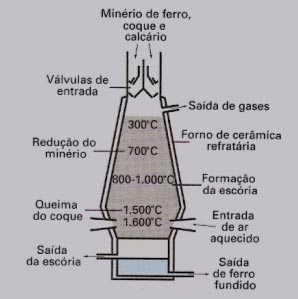
\includegraphics[width=0.85\textwidth,height=0.65\textwidth]{altoforno}
   \caption*{Fonte: Não lembro}
   \label{forno}
\end{figure}

\end{document}
%%% Local Variables:
%%% mode: latex
%%% TeX-master: t
%%% End:
